\section{CutOut}

Cutout, bir görüntünün belirli bir bölümünü rastgele kesip maskeler ve modelin bu eksik bilgiyle çalışmasını sağlar. Bu, modelin eksik bilgiye karşı dayanıklı hale gelmesine yardımcı olur. Veriyi bozarak, modele daha zorlu öğrenme örnekler sunar ve modelin sadece belirli bölgelere değil, görüntünün tümüne bakmasını sağlar. Bu da, veri seti üzerinde daha iyi genelleme yapmasını sağlar.

Cutout yöntemi, bir görüntü üzerinde rastgele bir kare bölgenin "cutout" (kesilip çıkarılması) işlemine dayanır. Kare şeklinde bir bölge seçilir ve bu bölgeye sabit bir değer atanarak (genelde sıfır veya siyah) maskeleme yapılır. Bu işlem, modelin dikkatinin görüntünün tamamına yayılmasını zorlar, çünkü eksik bilgi ile öğrenmek zorunda kalır.

\subsubsection{Python Kodu}

\begin{lstlisting}[language=Python]
from art.defences.preprocessor import CutoutTensorFlowV2

cutout = CutoutTensorFlowV2(length=6, apply_fit=True, apply_predict=False)
cutout_train = cutout.forward(x=x_train, y=y_train)
\end{lstlisting}

\begin{figure}[h]
    \centering
    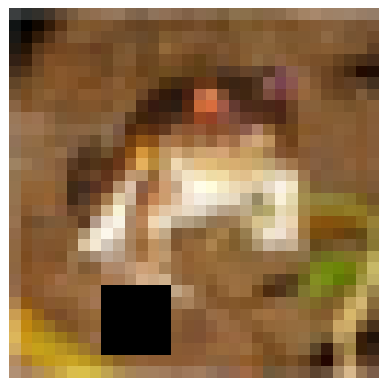
\includegraphics[width=0.3\textwidth]{images/cutout_example.png}
    \caption{}
\end{figure}

\newpage